% !Mode:: "TeX:UTF-8"
\chapter*{附录}
\label{appendix-figures}
\addcontentsline{toc}{chapter}{附录}

\begin{figure}[h!]
    \centering
    \begin{tabular}{cc}
        \subfigure[圆柱体体数据]{
            \label{cylinder_raw}
            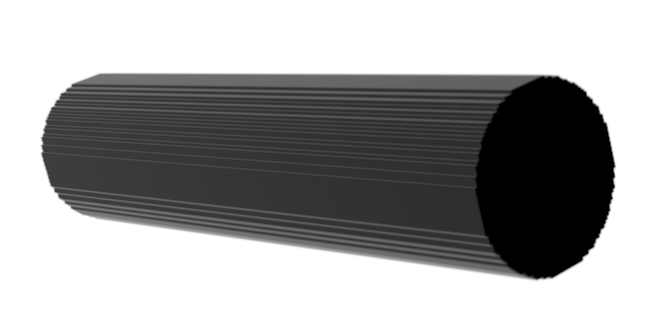
\includegraphics[width=.30\textwidth]{figure/other_test/cylinder_raw.png}
        } \hspace{4em} &
        \subfigure[圆柱体骨架]{
            \label{cylinder_skel}
            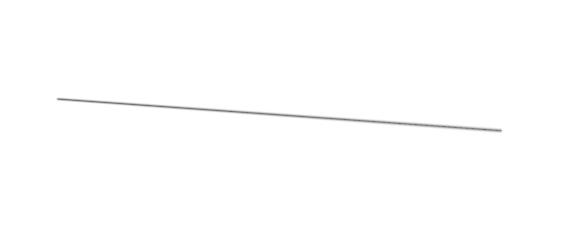
\includegraphics[width=.30\textwidth]{figure/other_test/cylinder_skel.png}
        } \\
        
        \subfigure[圆环体数据]{
            \label{donut_raw}
            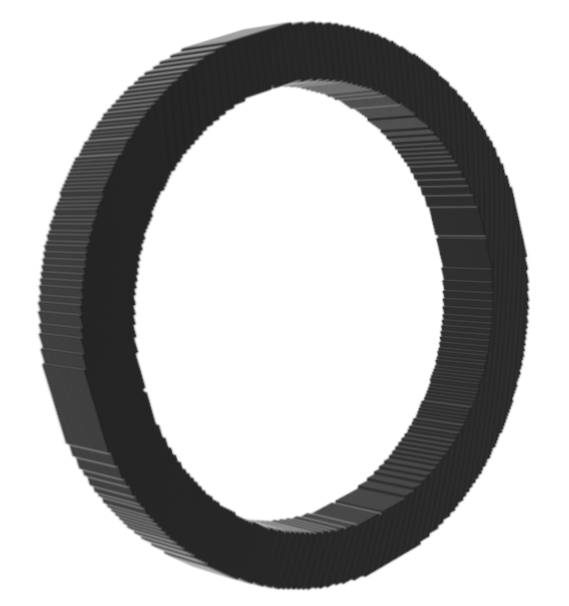
\includegraphics[width=.30\textwidth]{figure/other_test/donut_raw.png}
        } \hspace{4em} &
        \subfigure[圆环骨架]{
            \label{donut_skel}
            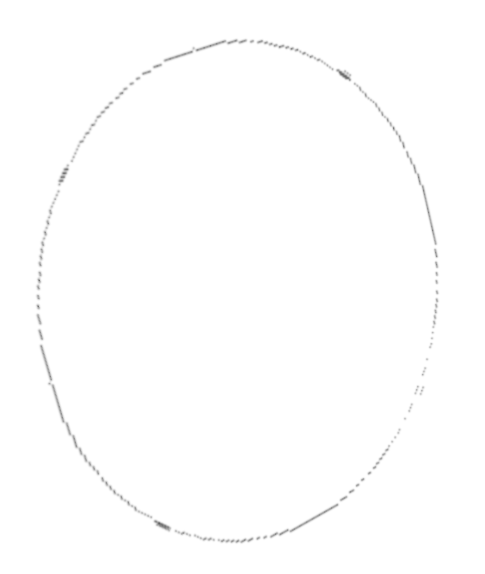
\includegraphics[width=.30\textwidth]{figure/other_test/donut_skel.png}
        } \\
        
        \subfigure[螺旋体数据]{
            \label{spiral_raw}
            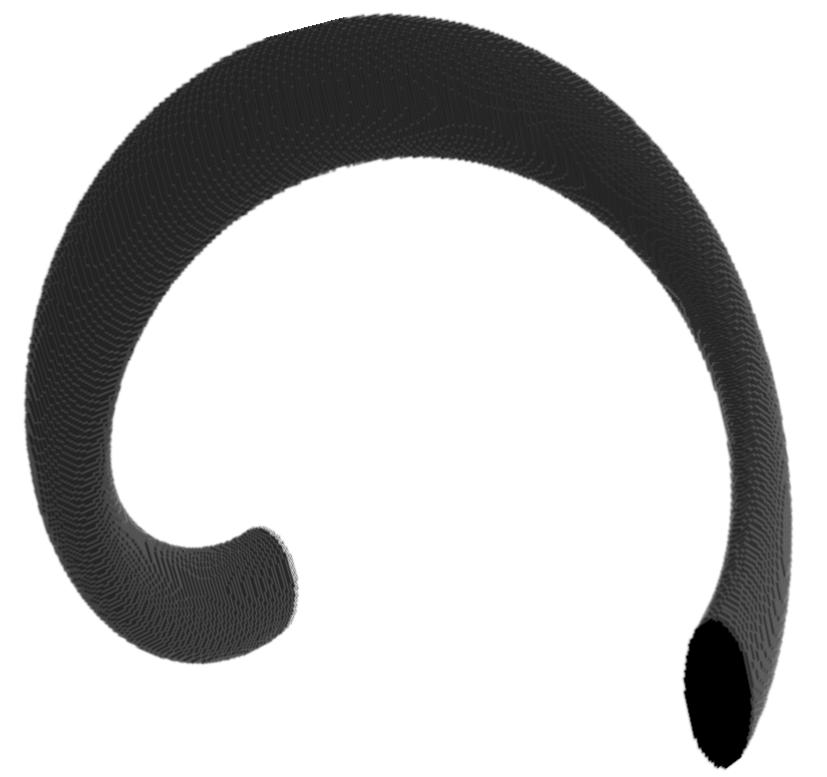
\includegraphics[width=.30\textwidth]{figure/other_test/spiral_raw.png}
        } \hspace{4em} &
        \subfigure[螺旋骨架]{
            \label{spiral_skel}
            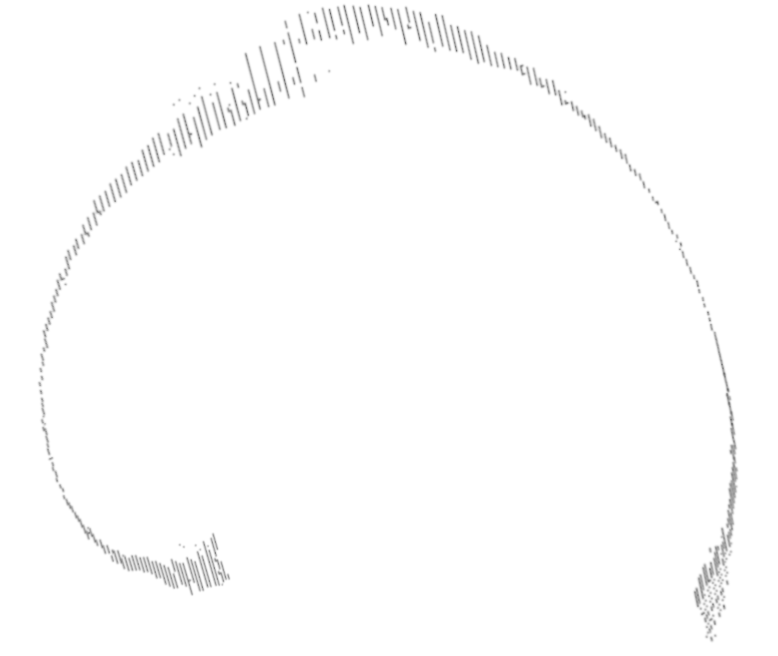
\includegraphics[width=.30\textwidth]{figure/other_test/spiral_skel.png}
        } \\
    \end{tabular}
    \caption{其他测试数据结果}
    \label{test-other-result-2}
\end{figure}
\cleardoublepage
